\chapter{Identificação de Padrões e Modelos de Previsão}
\label{chap:modelos}

\section{Identificação de Padrões por Clustering}
A análise exploratória do capítulo anterior revelou relações diretas entre pares de variáveis. Para procurar padrões mais complexos, que envolvam várias variáveis ao mesmo tempo, o grupo recorreu a aprendizagem não supervisionada. Esta parte foi implementada no \textit{script} \texttt{clustering.py}.

\subsection{Método Utilizado}
O algoritmo escolhido foi o \textit{K-Means}~\cite{geron}, por ser simples de interpretar e adequado a variáveis numéricas. Foram usadas como entrada cinco características relevantes para descrever o perfil dos pacientes e o seu resultado: idade, peso inicial, motivação, adesão média e variação de peso aos seis meses.

Antes da aplicação do algoritmo, todas as variáveis foram padronizadas com o \textit{StandardScaler}. Este passo é necessário porque o \textit{K-Means} se baseia em distâncias, e sem padronização as variáveis de maior escala, como o peso, dominariam o cálculo face a variáveis de menor escala, como a motivação. O número de grupos foi fixado em quatro, com o objetivo de identificar quatro perfis distintos de pacientes.

\subsection{Perfis Encontrados}
A tabela \ref{tab:clusters} resume os quatro grupos identificados.

\begin{table}[h]
\centering
\begin{tabular}{|c|r|c|c|c|c|}
\hline
\textbf{Grupo} & \textbf{Pacientes} & \textbf{Idade} & \textbf{Motivação} & \textbf{Adesão} & \textbf{Perda de peso} \\
\hline
0 & 842 & 31,3 & 0,78 & 85,7\% & $-27,8$ kg \\
1 & 744 & 56,9 & 0,79 & 85,5\% & $-22,2$ kg \\
2 & 642 & 44,9 & 0,55 & 59,9\% & $-13,9$ kg \\
3 & 5 & 42,0 & 5,00 & 79,2\% & $-23,8$ kg \\
\hline
\end{tabular}
\caption{Perfil médio de cada grupo identificado por \textit{clustering}.}
\label{tab:clusters}
\end{table}

A leitura dos três grupos principais conta uma história clara. O grupo 0 reúne os pacientes mais jovens, com idade média de 31 anos, alta adesão e a maior perda de peso. O grupo 1 reúne pacientes mais velhos, com idade média de 57 anos, com a mesma motivação e adesão dos mais jovens, mas com menor perda de peso. Esta diferença entre os grupos 0 e 1, com comportamento semelhante mas resultados diferentes, é coerente com o efeito da idade no metabolismo. O grupo 2 reúne os pacientes com motivação e adesão mais baixas, e é, como seria de esperar, o que perde menos peso.

A figura \ref{fig:clusters} mostra a distribuição dos pacientes segundo o peso inicial e a variação de peso, com cada grupo representado por uma cor. O gráfico permite ainda observar a presença de dois pontos isolados, com variações de peso próximas de mais e menos 100 kg, que correspondem a valores extremos não tratados pelo \textit{capping}, uma vez que este foi aplicado apenas às variáveis de idade, peso e altura.

\begin{figure}[h]
\centering
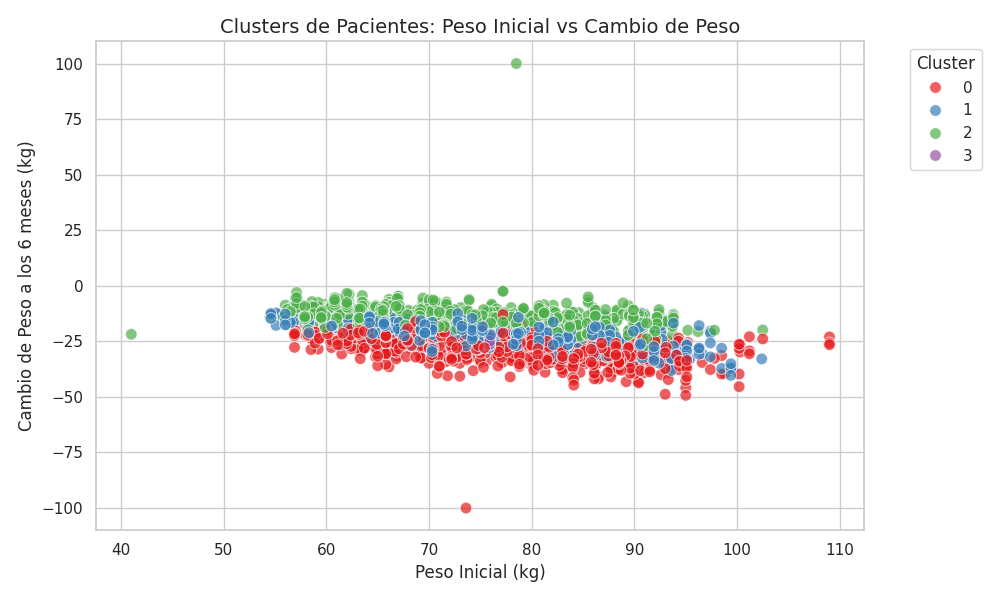
\includegraphics[width=0.85\textwidth]{clusters_peso.png}
\caption{Grupos de pacientes segundo o peso inicial e a variação de peso.}
\label{fig:clusters}
\end{figure}

\subsection{O Grupo Anómalo e a Qualidade dos Dados}
O grupo 3 merece destaque próprio. Contém apenas cinco registos e distingue-se por um valor de motivação de exatamente 5,0, enquanto todos os outros pacientes apresentam valores entre 0,15 e 0,99. Este valor não corresponde a pacientes extraordinariamente motivados, mas a um erro na introdução dos dados. Estes registos foram provavelmente preenchidos numa escala de 1 a 5, em vez da escala de 0 a 1 usada no resto do conjunto.

O facto de o \textit{K-Means} ter isolado automaticamente estes cinco registos num grupo próprio é, em si, um resultado relevante. Mostra que as técnicas de \textit{clustering}, para além de identificarem perfis de pacientes, funcionam também como uma ferramenta de deteção de problemas de qualidade dos dados que tinham passado despercebidos nas fases anteriores. Este foi um achado útil que o grupo registou para discussão.

\section{Aplicação de Modelos de Previsão}
A última fase de análise consistiu na aplicação de modelos de aprendizagem supervisionada, implementados no \textit{script} \texttt{predictive\_modeling.py} com recurso à biblioteca \textit{scikit-learn}~\cite{scikit}. O objetivo foi prever a variável \texttt{weight\_change\_kg\_6m}, ou seja, a quantidade de peso perdido ao fim de seis meses, tratando o problema como uma regressão.

\subsection{Seleção de Variáveis e Prevenção de Data Leakage}
A seleção das variáveis preditoras foi a decisão mais importante desta fase. Em primeiro lugar, foram removidas as colunas de identificação, como os identificadores de paciente, dieta e nutricionista, por não terem qualquer valor preditivo.

Em segundo lugar, e mais importante, foram removidas as variáveis que só são conhecidas durante ou depois do programa de dieta, nomeadamente a adesão média, o rácio de adesão, a motivação registada durante o programa e o índice do programa. A razão para esta remoção é evitar um problema conhecido como \textit{data leakage}. Se o modelo usasse a adesão para prever a perda de peso, estaria a usar informação que, na prática, ainda não existe no momento em que a previsão é útil, isto é, antes de a dieta começar. Um modelo treinado com essa informação teria um desempenho aparentemente excelente, mas seria inútil numa situação real. Ao remover estas variáveis, o grupo garantiu que o modelo só usa informação disponível à partida: características do paciente, da dieta e do nutricionista.

As variáveis categóricas restantes foram transformadas em variáveis numéricas através de codificação \textit{one-hot}. O conjunto final de características ficou com 33 colunas.

\subsection{Treino e Avaliação}
Os dados foram divididos em conjunto de treino, com 80\% das linhas, e conjunto de teste, com os restantes 20\%. Foram treinados três modelos de naturezas diferentes: uma regressão linear, uma \textit{random forest} e um \textit{gradient boosting}. A tabela \ref{tab:reg} apresenta os resultados no conjunto de teste, medidos pelo erro quadrático médio, pela sua raiz e pelo coeficiente de determinação.

\begin{table}[h]
\centering
\begin{tabular}{|l|c|c|c|}
\hline
\textbf{Modelo} & \textbf{MSE} & \textbf{RMSE (kg)} & \textbf{$R^2$} \\
\hline
Regressão linear & 18,54 & 4,31 & 0,655 \\
\textit{Random forest} & 10,98 & 3,31 & 0,796 \\
\textit{Gradient boosting} & 11,69 & 3,42 & 0,783 \\
\hline
\end{tabular}
\caption{Desempenho dos modelos de regressão no conjunto de teste.}
\label{tab:reg}
\end{table}

Os modelos baseados em árvores, a \textit{random forest} e o \textit{gradient boosting}, tiveram um desempenho claramente superior ao da regressão linear. A \textit{random forest} foi o melhor modelo, com um coeficiente de determinação de 0,796 e um erro médio de cerca de 3,3 kg. A análise destes resultados é aprofundada no capítulo seguinte.
